% Ausarbeitung SAJ 
% FH Augsburg 
%
%
%
%
\documentclass[titlepage, 12pt,a4paper]{scrartcl}
%scrartcl
\usepackage[ngerman]{babel}
%\usepackage[latin1]{inputenc}
\usepackage[T1]{fontenc}
\usepackage{ucs}            % Eventuell benötigt
\usepackage[utf8x]{inputenc}

\usepackage{setspace}           % Paket fuer den Zeilenabstand
\onehalfspacing                 % Setzt den Zeilenabstand auf 1.5

\usepackage{graphicx}
\usepackage{listings}
\usepackage[hyphens]{url}
%\usepackage{breakurl}
\usepackage{hyperref}
\usepackage[usenames]{color}
\definecolor{light-gray}{gray}{0.90}
\usepackage[fixlanguage]{babelbib}
\usepackage{listings}
%\lstset{numbers=left, numberstyle=\tiny, numbersep=5pt}
%\lstset{language=Perl}
\lstloadlanguages{bash,XML,HTML, PHP}
\selectbiblanguage{german}
\usepackage{makeidx}
%\usepackage{pifont}
\makeindex
%\usepackage{fancyhdr}
%\setlength{\headheight}{15.2pt}
%\pagestyle{fancy}


\author{Stephan Urban \& Andrés Cuartas}
\title{- Ausarbeitung - \\ Softwarearchitekturen in Java \\}
%\date{11-Dez-2007}

\pagestyle{myheadings}
\markright{Urban \& Cuartas}
\lstset{
	inputencoding=utf8x,
	extendedchars=\true,
	language=XML,
	basicstyle=\tiny,
	keywordstyle=\bfseries\color{green},
	identifierstyle=,
	%commentstyle=\color{gray},	
	%stringstyle=\itshape\color{darkred},
	numbers=left,
	numberstyle=\tiny,
	stepnumber=1,
	breaklines=true,
	frame=none,
	showstringspaces=false,
	tabsize=4,
	backgroundcolor=\color{light-gray},
	captionpos=b,
	float=htbp,
	frameround=fttt
}


%\lstset{language=XML, stringstyle=\ttfamily, tabsize=2, basicstyle=\small, breaklines=true, backgroundcolor=\color{light-gray}, frameround=fttt}
%              
% WORKAROUND, damit lstlistoflistings funktioniert: 
% Quelle: http://www.komascript.de/node/477
%
\makeatletter% --> De-TeX-FAQ
\renewcommand*{\lstlistoflistings}{%
  \begingroup
    \if@twocolumn
      \@restonecoltrue\onecolumn
    \else
      \@restonecolfalse
    \fi
    \lol@heading
    \setlength{\parskip}{\z@}%
    \setlength{\parindent}{\z@}%
    \setlength{\parfillskip}{\z@ \@plus 1fil}%
    \@starttoc{lol}%
    \if@restonecol\twocolumn\fi
  \endgroup
}
\makeatother% --> \makeatletter 

\begin{document} 

\maketitle

\newpage
\tableofcontents
\newpage

\section{Einführung}
Im Rahmen des Wahlpflichtfaches Softwarearchitekturen in Java haben wir die
Aufgabe unser Teilprojekt, den Spezialbereich „Java Server Faces“ in einer
Ausarbeitung zu dokumentieren. 

Im Folgender Ausarbeitung werden wir auf die Teilbereiche bzw. Milesteones
eingehen. Einen überblick über den übertragenen Spezialbereich geben und
Probleme und Lösungen darstellen, auf die wir gestoßen sind. 

\section{Domain Modell}
Nachdem wir das Teilgebiet „Lehrevaluation“ zugelost bekamen, machten wir uns
erstmal Gedanken darüber wie während des Verlaufs unserer Studienzeit bisher
Lehrevaluationen durchgeführt wurden. Evaluationen verliefen alle auf ähnliche
Weise, dabei bekommen Studenten immer einen Fragebogen der im Normalfall so
aufgeteilt ist, dass Noten vergeben werden können. Ein Teilbereich für den
Gesamteindruck einer Vorlesung, ein anderer über Fachliche Aspekte und im
dritten Teil kann der Student Kommetare bzw. Verbesserungsvorschläge an dern
Professor richten. Natürlich verläuft die Evaluierung anonym und in Papierform
ab.

Unsere Aufgabe bestand darin diesen Verlauf zuerst durch Anforderungen in Form
von Userstories umzusetzen, um ein Gefühl dafür zu bekommen, was bei einer
Evaluierung auf der Seite der Studenten gefordert wird und auch was ein
Professor für Administrationsaufgaben hat, wenn er eine  Evalutaion erstellt.
Auch sollte ein Administrator berücksichtigt werden, der über alle nötigen
Rechte und die größte Übersicht auf Lehrevaluationen erhält. 

Mit Hilfe folgender Userstories haben wir die grundsätzlichen Anforderungen an
das System herausgearbeitet und uns einen Überblick verschafft.  

\begin{enumerate}
\item Student: 
\begin{enumerate} 
\item Auswahl verschiedener Fächer, abhängig vom Studiengang, bei denen entweder eine Evaluation möglich ist, bzw. diese abgeschlossen ist.
\item Anzeige der Evaluationsergebnisse
\item Student hat Evaluationsbogen vor sich und im ersten Abschnitt für Kriterien Noten vergeben
\item Im zweiten Abschnitt kann Lob/Kritik oder Anmerkungen schriftlich äußern
\item Am Ende wird eine Zusammenfassung angezeigt, die noch editierbar ist
\item Speichern/Übermitteln der Evaluation 
\end{enumerate}

\item Kriterien aus dem ersten Teil sind:

\begin{enumerate}
\item Niveau
\item Material
\item Vermittlung des Stoffs
\item Praxisbezug
\item Roter Faden
\item Eingehen auf Fragen
\item Arbeitsaufwand
\item Übungen
\item Gesamtbeurteilung der Veranstaltung 
\end{enumerate}

\item Professor: 
\begin{enumerate}
\item Beim Klick auf Evaluation starten, wird diese für alle Studenten
\item freigeschaltet. Beim Klick auf editieren werden, 
die Durchschnittswerte der einzelnen Noten angezeigt, sowie alle
schriftlichen Bewertungen. Die schriftlichen Bewertungen können auf dieser
Seite einzeln zur Veröffentlichung freigegeben bzw. wieder entfernt werden.

\end{enumerate}

\item Mitarbeiter: 
\begin{enumerate}
\item Kann im Grunde alles, was der Professor kann, im werden alle Evaluationen
aufgelistet.
\end{enumerate}

\end{enumerate}

In dieser Phase gab es insofern Probleme, dass wir eingrezen mussten wie
flexibel bzw. wie tief die einzelnen Personen das System betrachten dürfen. Es
musste also ein Mittelweg gefunden werden, welche fundamentalen funktionen das
System bieten sollte und was, um die Übersicht und die Umsetzung des
Teilgebiets so funktional und einfach wie möglich zu halten, weggelassen werden
sollte. Hierbei ist die Entscheidung gefallen den Mitarbeiter entfallen zu
lassen, weil dieser im Vergleich zum Professor nicht mehr Funktionalität inne
hat. 
\section{Klassenentwurf}
Um so effizient wie möglich am Projekt arbeiten zu könnnen, wurde überlegt, wie
die Zusammenarbeit durchgeführt werden sollte. Zu diesem Zeitpunkt hatten
wir die Möglichkeit GoogleWave einzusetzen. Zuvor war die Überlegung
Informationen im Projektwiki festzuhalten bzw. dort direkt zu bearbeiten. Die
Entscheidung fiel dann so, dass prototypisch unter GoogleWave Informationen
ausgetauscht wurden und wenn etwas dann für die Allgemeinheit festzuhalten war,
diese Informationen ins Wiki übeartragen wurde. 

\begin{figure}[h]
\begin{center}
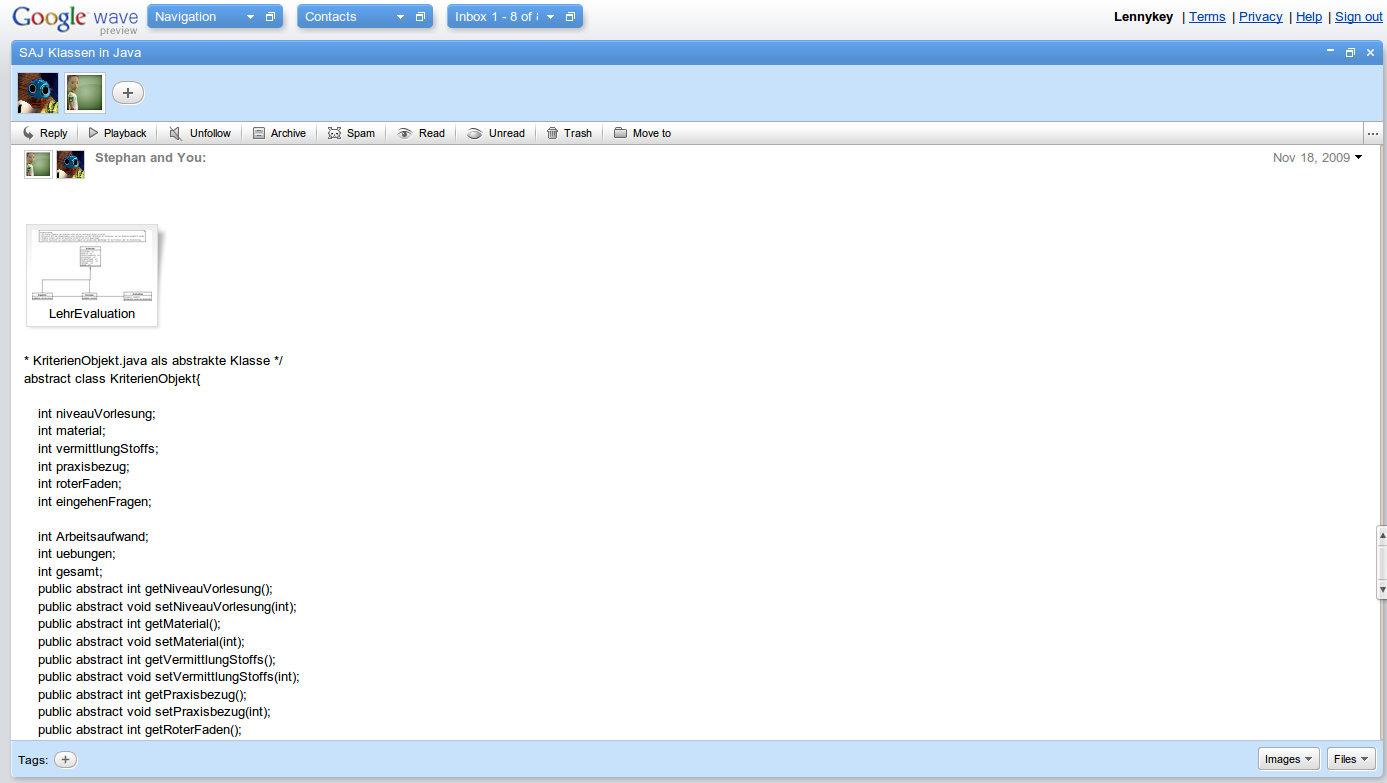
\includegraphics[width=15cm, height=12cm]{bilder/googleWave.png}
\caption{Google Wave}
\label{googleWave}
\end{center}
\end{figure}

So wurden Überlegungen des Klassenentwurfs unter GoogleWave diskutiert,
Teilergebnisse und fertige Klassendiagramme dann auf das Trac-Wiki
übertragen. Der Vorteil dieser Methode ist es, dass so die Gedanken und
Ideeenaustausch online und in echtzeit stattfinden konnte. So konnten Treffen
und die Fahrten in die FH entfallen und effizienter Zeit in das Projekt
einfließen.

So entstand ein Grobentwurf der Klassen zuerst in der Diskussion und mit Hilfe
von Opensource UML-Tools wie Umbrello, da unsere studentische Lizenzen für
VisualParadigm bereits abgelaufen waren. Leider lief Umbrello nicht so stabil,
so dass ein alternatives Tool gesucht wurde. Die Wahl fiel dann auf „DIA“, um
unsere Idee für das Klassendiagramm zu visualisieren, welches auf für
Netzwerkdiagramme benutzt werden kann. Da wir unter Java noch nicht so viel
Erfahrung mitbrachten erstellten wir dann aus dem Diagramm erstmal die Klassen
mit Hilfe von C++ Code, das aber ohne weiter Probleme später in Java-Code
umgeschrieben werden konnte.

\begin{figure}[h]
\begin{center}
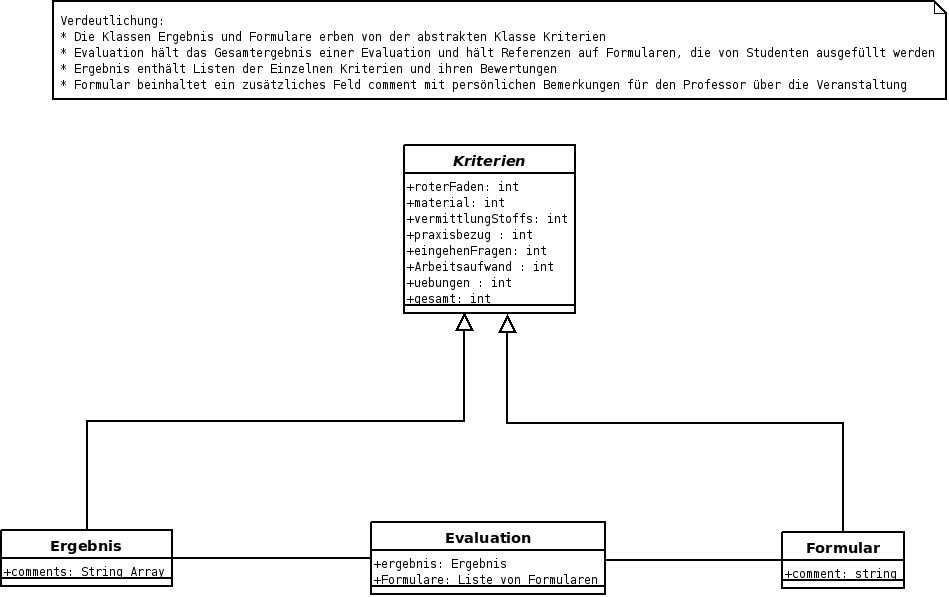
\includegraphics[width=15cm, height=12cm]{bilder/LehrEvaluation.png}
\caption{Klassenentwurf}
\label{Klassen}
\end{center}
\end{figure}

Die ersten Entwürfe wurden dabei mehrmals überarbeitet bis ein Klassendigramm
entstand, welches unsere Bedürnisse an das System einigermaßen gedeck hat.
Dabei ist uns erst nach Durchsicht von Prof. Meixner aufgefallen, dass
Kommentare der Studenten zu doppelt gespeichert wurden und zwar in einem
Formular selbst, wie auch in der Liste der Ergebnisse. Im
Klassendiagramm wurde auch noch nicht berücksichtigt, dass die Ergebnisse
Durchschnittswerte darstellen, die aber in der Parent-Class als Integer Werte
deklariert wurden. Es wurden weiterhin Redundanzen in den Setter und Getter
Methoden festegestellt und der Bezug einer Evaluierung zu einer
Lehrveranstaltung fehlte noch. Zu diesem Zeitpunkt waren die DAOs und die
Serviceschicht in Planung so dass das Weiterleiten der Ergebnisse an die
Serviceschicht und somit an die Weboberfläche noch nicht möglich war. 

Die obengenannten Punkte konnten dann ohne weitere Probleme behoben werden und
so konnten wir die Implementierung der DAOs und der Serviceschicht angehen. 

\section{Persistenz}
Um die Ergebnisse einer Evaluation zu sichern, wurde überlegt, was wirklich
persistent gehalten werden sollte, um Redundanzen so gering wie möglich zu
halten.

So ist es in unserem Teilprojekt nicht wichtig die Formulare mit samt den
Kommentaren einzeln zu speichern. Denn falls ein Formular bearbeitet wird,
werden die Durchschnittswerte in die Evaltuation verrechnet. Diese
Durchschnittswerte werden nach Beendigung der Evaluation nicht mehr verändert in
Folge werden nur dieser Ergebnisse persistent gehalten und nicht die enzelnen
Formulare. Auch die Kommentare zu der Evaluation werden in Verbindung zur
diesen gespeichert. Ein weiterer Vorteil ist, dass so, bei der Ausgabe,
die Ergebnisse nicht aus den einzelnen Formularen immer wieder neu berechnet
müssen sondern sofort zur Verfügung stehen und somit schneller zurückgegeben
werden können, z.B. an die Weboberfläche.

Ein Nachteil dabei ist, dass die Transparenz nicht mehr gewahrt bleibt, da die
Einzelergebnisse/Formulare nicht mehr existieren. Es sei denn die Formulare
werden in Papierform zur Verfügung gestellt und dann erst ins System
eingegeben, aber dieser Umweg soll durch dieses Teilprojekt vermieden werden
und jeder Student sollte die Möglichkeit bekommen online Formulare auszufüllen.


\section{Weboberfläche}
Mit Hilfe von JavaServerFaces ist es leicht möglich auf die die Methoden und
Attribute der Serviceschicht zuzugreifen. Deswegen haben wir uns dafür
entschieden für die Weboberfläche JSF einzusetzen. Auch aus den Guten
Erfahrungen während der Recherche zu unserem Spezialthema für die Vorlesung. 

\section{JUNIT Tests}

\section{Java Server Faces}
Am anfang der Einarbeitung war es schwierig die vorhandenen Beispiele aus
Büchern bzw. dem Internet zum Laufen zu kriegen, auch deswegen, da es an
Erfahrung mit Eclipse fehlte. Im laufe des „Try and Error“ die richtige
Konfiguration unter Eclipse einzustellen, konnte letztendlich eine
Beispielanwendung zum Laufen gebracht werden. Dabei gibt es zwei verschiedene
Ansätze. 

Erster Ansatz, man bindet unter Eclipse z.B. dem Tomcat Webserver ein und legt
alle benötigten Bibliotheken in den „WEB-INF/lib“ ordner. Folgende Dateien
sollten für ein funktionierendes Java Server Faces Projekt eingebunden
bzw. kopiert werden. Die
JSTL\footnote{http://download.java.net/maven/1/jstl/jars/jstl-1.2.jar}
Implementation, leider funktioniert die neuste Implementation, die man z.B. aus
dem Mojarra\footnote{https://jstl.dev.java.net/download.html} Projekt
runterladen nicht, weil ein paar Libraries fehlen ohne die man nicht auf Java
Server Pages zurückgreifen kann, um mit diesen zu arbeien. Darüberhinaus ist es
noch nötig, sich für eine JSF Implementation zu entscheiden. Für den Anfang
reicht es auf die Mojarra Implementation zurückzugreifen. Benötigt man weitere
Funktionalität bzw. weitere JSF-Tags die mehr Funktionalität bieten, lohnt es
sich mit Apache MyFaces auseinander zu setzen. 

Der andere Ansatz ist, die benötigten Bibliotheken als UserLibraries unter
Eiclipse einzubinden und diese dann in den Java Build Path mit aufzunehmen.
Darüberhinaus sollte auch beachtet werden, unter „Properties->Java EE
Module Dependencies“ die benötigten Bibliotheken zur Laufzeit einzubinden.

\begin{figure}[h]
\begin{center}
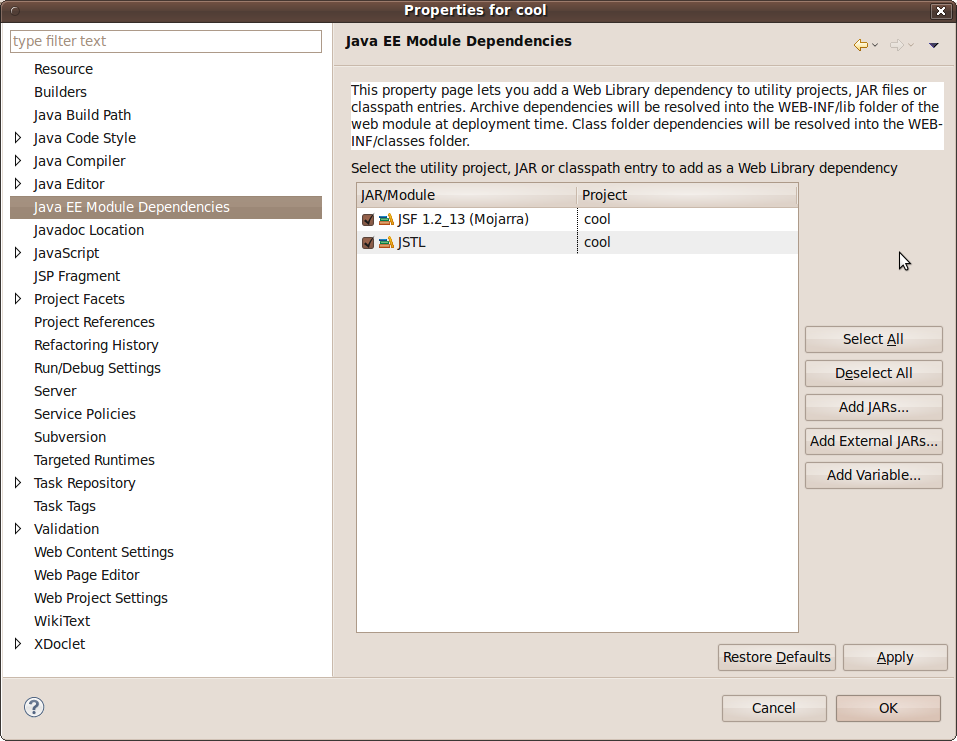
\includegraphics[width=15cm, height=10cm]{bilder/Properties.png}
\caption{Properties}
\label{properties}
\end{center}
\end{figure}

Wenn dieser Schritt ausgelassen wird, was im Laufe der Konfiguration
und mangels Erfahrung mit Eclipse oft passiert ist, kann der Webserver nicht
auf die benötigten Bibliotheken zugreifen und somit das Projekt nicht
ausführen. 

Folgende Fehlermeldungen können dann in der Fehlerkonsole unter Eclipse
angezeigt werden:


\begin{verbatim}
SCHWERWIEGEND: Error configuring application listener of class
com.sun.faces.config.ConfigureListener
java.lang.ClassNotFoundException: com.sun.faces.config.ConfigureListener

org.apache.catalina.core.StandardContext listenerStart
SCHWERWIEGEND: Skipped installing application listeners due to previous
error(s)

org.apache.catalina.core.StandardContext start
SCHWERWIEGEND: Error listenerStart

\end{verbatim}

Wobei die angegebenen Java Klassen nicht gefunden werden, die sich z.B. in den
JSF Implementierungen oder in der JSTL befinden. 




Hier Netbeans Teil :-)



\end{document}
